\pagenumbering{arabic}

\section{概率的悖论}

\subsection{悖论}

悖论是一逻辑学术语,指那些会导致逻辑矛盾的命题.如果承认这个命题成立,就
可推出它的否定命题成立;反之,如果承认这个命题的否定命题成立,又可推出这个命题
成立.像这样自相矛盾的命题就是悖论.
\par 悖论是表面上同一命题或推理中隐含着两个对立的结论,而这两个结论都能自圆其
说.悖论的抽象公式就是:如果事件A发生,则推导出非A,非A发生则推导出A.
\par 古今中外有不少著名的悖论,它们震撼了逻辑和数学的基础,激发了人们求知和精
密的思考,吸引了古往今来许多思想家和爱好者的注意力.解决悖论难题需要创造性的
思考,悖论的解决又往往可以给人带来全新的观念.

\subsection{贝特朗悖论}
“在一个圆内任意选一条弦,这条弦的弦长长于这个圆的内接等边三角形的边长的
概率是多少?”

\subsubsection{问题提出}
几何概率是十九世纪末新发展起来的一门学科,使很多概率问题的解决变得简单而
不用运用微积分的知识.而正当几何概型正如火如荼的发展时,法国学者贝特朗于1899
年针对几何概念提出了这样一个“简单”的问题,并在当时数学界引起了轩然大波.按照几何概率的定义进行计算,
竟然可以求得3个不同的概率,这与概率的性质是背道而驰的.这就是后来人们熟知的贝特朗悖
论,矛头直指几何概率概念本身.

\subsubsection{三种解法}
首先,关于几何概型和几何概率,有如下定义,若随机试验$E$具有以下特点:
\par (1) 样本空间是直线或二维、三维空间中的度量有限的区间或区域;
\par (2) 样本点在其上是均匀分布的(即所有基本事件是等可能的).\\
则这样的随机试验称为几何概型.在几何概型中,若样本空间$\Omega$所对应区域的度量
为$L(\Omega)$,且事件$A$的度量为$L(A)$,则事件$A$的概率为
\[
	P(A) = \dfrac{L(A)}{L(\Omega)}.
\]
在贝特朗问题提出时,贝特朗就提出了3种经典的解法:

\paragraph*{方法一} 任意弦交圆周于两点,不妨将弦的一段$A$固定,问题化为在圆周上任取另一端
点$B$.这时,样本空间$\Omega$为圆周上任一点,假设任一点的选取具有等可能性.如图1.1(a)
所示,以$A$为顶点做一等边三角形$AMN$,显然弦$AB$的长度大于$\sqrt{3}$当且仅当端点$B$
落在$\wideparen{MN}$上.而$\wideparen{MN}$的长为整个圆周的$\dfrac{1}{3}$,于是所求概率为$\dfrac{1}{3}$.

\paragraph*{方法二} 如图1.1(b)所示,不妨只考虑与直径$MN$垂直的弦,样本空间$\Omega$为$MN$上任
一点,假设弦$AB$的中点在$MN$上是等可能的.当且仅当弦$AB$与圆心的距离小于$\dfrac{1}{2}$
时,弦$AB$的长度大于$\sqrt{3}$,于是所求概率为$\dfrac{1}{2}$.

\paragraph*{方法三} 如图1.1(c)所示,弦被其中点唯一确定,假设弦的中点在圆周内是等可能的.当
且仅当弦$AB$的中点在半径为$\dfrac{1}{2}$的同心圆内时,弦$AB$的长度大于$\sqrt{3}$,此小圆面积为
大圆面积的$\dfrac{1}{4}$,于是所求概率为$\dfrac{1}{4}$.

\begin{figure}[thbp!]
	\centering
	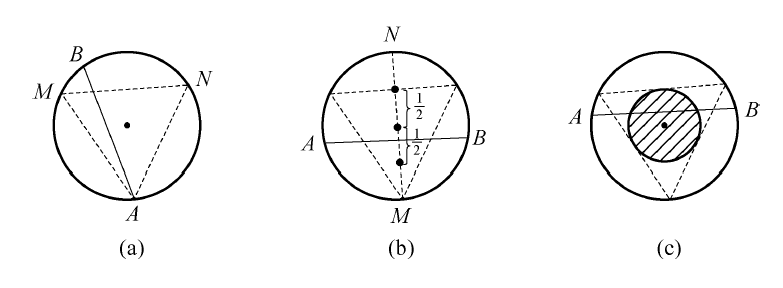
\includegraphics[width=0.8\linewidth]{figure/circ.png}
	\caption{}
	\label{fig:circ}
\end{figure}

由于在取弦时采用了3种不同的等可能假设,对3种不同的随机试验得到了3种不
同结果,通过分析这3种结果均正确.而这这严重违背了常理.

\subsubsection{观点争执}
贝特朗问题之所以出现3种不同的答案,是因为人们观察随机试验的基本结果的角
度不同,同时对基本结果的等可能性假设也有不同的理解.

\par 然而,仍然有不少学者对此持怀疑态度,并根据自己对问题的理解以及自己特有的
思维方式,钟情于其中的某种解法,想方设法寻找其他解法的瑕疵,推翻其他解法的合理
性,从而认为贝特朗悖论并不奇,答案其实是唯一的.